\DiaryEntry{Cubic Equations - in progress}{2018-03-05}{Complex Analysis}


Based / inspired by Tristan Needdham, "Visual Complex Analysis".


We want to solve the cubic equation

\bee
y = x^3 + a x^2 + b x + c = 0
\eee

The inflection point (that is where $y'' = 0$) is given by: $y' = 3x^2 + 2ax + b, y'' = 6x + 2a$ and from this follows that the inflection point is $x = -a / 3$. Exercise V/1 in the book is to show that the quadratic term of the equation above vanishes when we substitute $x \rightarrow u - a_0/3$. We can simply perform the substitution and arrive at 

\bee
y = (u-a/3)^3 + a(u-a/3)^2 + b(u-a/3) + c = \cdots + u^3 + Bu + C
\eee

where $A,B,C$ are some constants calculated via e.g. Maxima as follows.

\begin{verbatim}
(%i1)	ratsimp((u-a/3)^3+a*(u-a/3)^2 + b*(u-a/3) + c);
(%o1)	(27*u^3+(27*b-9*a^2)*u+27*c-9*a*b+2*a^3)/27
\end{verbatim}

This shows that we only have to deal with equations with $a=0$. For whatever reasons, we write these equations as

\bee
y = x^3 - 3px - 2q
\eee

\subsection{Simple Cases}

Consider first the case when $q=0$.

\bee
y = x^3 - 3px = 0
\eee

which we can factor as $y = x(x^2 - 3p) = 0$ and we have the three solutions $x_0 = 0, x_{1,2} = \pm \sqrt{3p}$.

The curve fulfills the following symmetry: $y(-x) = -y(x)$.

We can see more clearly what happens by calculating the position of local minimums and maximums. Assume that $p>0$, $y' = 3x^2 - 3p = 0$ and therefore $x = \pm \sqrt{p}$. With $y'' = 6x$, $y''(\sqrt{p}) > 0$ and therefore $x = \sqrt{p}$ is a local minimum. We have $y''(-\sqrt{p}) < 0$ and therefore $x = -\sqrt{p}$ is a local maximum. For large absolute values of $x$, the cubic term dominates and these considerations explain the following plot.

\begin{figure}[H]
	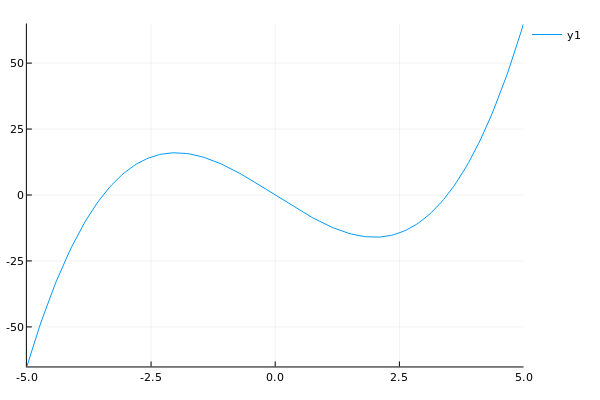
\includegraphics[scale=0.7]{images/cubic_01.png}
\end{figure}

\subsection{Complete Solution}

This is now exercise V/2

\todo{Solve the exercise}

What I don't get is this: How many roots does this give? I think from solving the quadratic equation, we get two (the $\pm$ before the square root). But then the cubic root should have 3 roots. Some of the stuff should cancel out, so that only three solutions remain.

 Btw, either there are three real solutions, or one real solution and two complex (conjugate) ones. A special case is that there is one (three-fold) solution.
 
 If we have $\sqrt[3]{A} = C$, then there are two other solutions as $\left(-\frac{1}{2} \pm \frac{1}{2}\sqrt{3}j\right)C$.


